\section{Kinematics}

\subsection{Reference frames}

\subsubsection{Rotation Matrix differential equation}

The following equation expresses how the reference frame moves as a function of its rotational velocity and the rotation matrix itself,

\begin{equation} \label{eq:rotation_ODE}
    \begin{aligned}
    \dot{R}^a_b = (\omega^a_{ab})^\times R^a_b \\
    \dot{R}^a_b = R^a_b(\omega^b_{ab})^\times
    \end{aligned}
\end{equation}

\subsubsection{Derivative}

The derivative of a vector depends on which frame it is differentiated with respect to as "velocity" is relative, following is an example involving position $r_p$ its derivative,

\begin{align} \label{eq:reference_frame_derivative}
    \begin{split}
        (v_p)_{x_by_bz_b} &\leftrightarrow {}^b\frac{d}{dt}(r_p)
        \\
        {}^o \frac{d}{dt}(\Vec{r}_p) &= {}^b\frac{d}{dt}(\Vec{r}_p) + \omega \times \Vec{r_p}
    \end{split}
\end{align}

This derived from derivative of $r^a = R^a_b r^b$ using Equation \eqref{eq:rotation_ODE}, where $\Dot{r}^i$ is vector $r$ differentiated with respect to a frame $i$,

\begin{align}
    \begin{split}
        \Dot{r}^a &= R^a_b \Dot{r}^b + \Dot{R}^a_b r^b
        \\
        &= R^a_b \begin{bmatrix}
            \Dot{r}^b + (\omega^b_{ab})^\times r^b
        \end{bmatrix}
        \\
        \frac{^ad}{dt} r &= \begin{bmatrix}
            \frac{^bd}{dt} r + \omega_{ab} \times r
        \end{bmatrix}
    \end{split}
\end{align}

%\begin{equation}
%    \Vec{a^i_c} 
%    = 
%    {}^i\frac{d}{dt}\Vec{v}_c 
%    = 
%    {}^b\frac{d}{dt}\Vec{v}_c + \Vec{\omega}_{ib} %\times \Vec{v}_c
%\end{equation}

\subsection{Linear Position}
\begin{figure}[H]
    \centering
    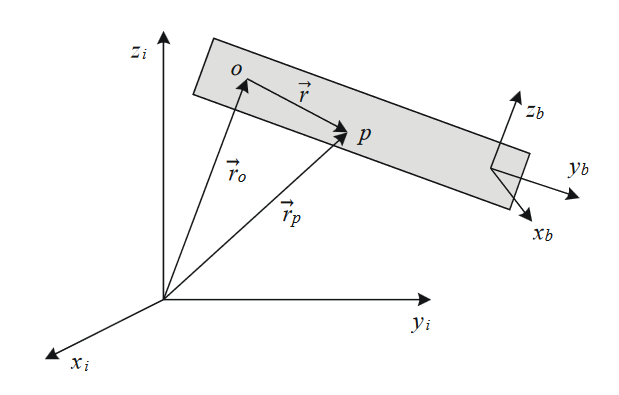
\includegraphics[scale=0.6]{figures/Rigid body configuration.png}
    \caption{1 stykk stiv kropp stjålet fra boka}
    \label{fig:rigid_body}
\end{figure}

In \autoref{fig:rigid_body} $\vec r_o$ is the position of the body in relation to the inertial frame $i$. 

Here $\vec r$ is the vector from $o$ to $p$ with coordinate vector $\mathbf{r}^b$ in the $b$ frame. This vector is given in the $i$ frame by
$\mathbf{r}^i = R^i_b\mathbf{r}^b$

\subsection{Linear Velocity}
The velocities of $o$ and $p$ in $i$ frame is given by
$$
\vec{v}_o:=\frac{^id}{d t} \vec{r}_o, \quad \vec{v}_p:=\frac{^id}{d t} \vec{r}_p
$$
Using $\vec r_p=\vec r_o+\vec r$ and the rule for differentiation in moving frames, we can express $\vec r_p$ as
$$
\vec{v}_p:=v_o+\frac{^bd}{d t} \vec{r}+\omega_{ib}\times \vec r
$$
where $\omega_{ib}$ is the angular velocity vector of frame $b$ relative to frame $i$ (see \autoref{fig:rigid_body} for how vectors are related).


%% OLD
% The linear velocity $v_B$ of body $B$ in frame $O$ is given by
% $$
% v_B=v_{O_B} + \dot r_{B/O_B}
% $$
% where $v_{O_B}$ is the velocity of the origin of the $B$-frame $O_B$ and $r_{B/O_B}$ is the position of the body $B$ in relation to the origin of the body frame $O_B$. (All vectors except $\dot r_{B/O_B}$ are in the origin frame $O$)

% The time derivative of the position vector $\dot r_{B/O_B}$ can be expressed as the sum of the velocity of the body in $B$-frame and the translational velocity due to angular velocity so that:
% $$
% v_B=v_{O_B}+v_{B/O_B}+\omega\times r_{B/O_B}
% $$
% where $\omega$ is the angular velocity of the body $B$

\subsection{Linear Acceleration}
Similar to the velocity vectors, the acceleration vectors are defined as
$$
\vec{a}_o:=\frac{^id^2}{dt^2} \vec{r}_o, \quad \vec{a}_p:=\frac{^id^2}{dt^2} \vec{r}_p
$$
(See \autoref{fig:rigid_body})
We define the angular acceleration vectors as
$$
\vec{\alpha}_o:=\frac{^id}{d t} \omega_{ib} = \frac{^bd}{d t} \omega_{ib}
$$
Replacing $\vec r_p=\vec r_o+\vec r$, we get
$$
\underbrace{\vec a_p}_{\text{acceleration of p}} = a_o +
\underbrace{\frac{^bd^2}{dt^2} \vec{r}_p}_{\text{second derivative of } \vec r \text{ in } b} + 
\underbrace{2\omega_{ib}\times \frac{^bd}{dt} \vec{r}}_{\text{Coriolis acceleration}} +
\underbrace{\alpha_{ib}\times \vec r}_{\text{Transversal acceleration}} +
\underbrace{\omega_{ib}\times(\omega_{ib}\times \vec r)}_{\text{Centripetal acceleration}}
$$
The acceleration of the frame $a_o$ can also be expressed as
$$
a_o=\frac{^id}{dt} \vec{v}_o = \frac{^bd}{dt} \vec{v}_o+ \omega_{ib}\times v_o
$$

% Taking the time-derivative of velocity we get the acceleration of body $B$ in the origin frame $O$:
% $$
% a_B=a_{O_B}+\alpha\times r_{P/O_B}+\omega\times(\omega\times r_{P/O_B})+2\omega\times v_B
% $$
% where $\alpha$ is the angular acceleration of $B$.

\subsection{Angular Velocity}
A vector $r$ undergoing uniform circular motion around a fixed axis satisfies
\begin{equation}
    \dot{r} = \omega \times r
    \label{eq:angular_velocity}
\end{equation}


\textbf{Rotation matrices:}
The kinematic differential equation of the rotation matrix is given by the two alternative forms
\begin{equation*}
    \begin{aligned}
    \dot{R}^a_b = (\omega^a_{ab})^\times R^a_b \\
    \dot{R}^a_b = R^a_b(\omega^b_{ab})^\times
    \end{aligned}
\end{equation*}
where $\omega^b_{ab}$ is the angular velocity vector of frame b relative of frame a expressed in frame b.

For a \emph{simple rotation}, the angular velocity vector $\vec{\omega}_{ab}$ is along the axis of rotation $\vec{k}$, and is given by
\begin{equation*}
    \begin{aligned}
    \vec{\omega}_{ab} = \dot{\theta} \vec{k}
    \end{aligned}
\end{equation*}

The angular velocity of the \emph{composite rotation} matrix $R^a_d = R^a_b R^b_c R^c_d$ is the sum of the angular velocities according to
\begin{equation}
    \begin{aligned}
    \vec{\omega}_{ad} = \vec{\omega}_{ab} + \vec{\omega}_{bc} + \vec{\omega}_{cd}
    \end{aligned}
    \label{eq:sum_of_angular_vel}  
\end{equation}

\textbf{Euler angles:}
When Euler angles are used the rotation matrix $R_{ad}$ from frame a to frame d is a composite rotation involving three simple rotations $R^a_d = R^a_b R^b_c R^c_d$ where
\begin{equation*}
    \begin{aligned}
    R^a_b = R_z(\psi),\; R^b_c = R_y(\theta),\; R^c_d = R_x(\phi)
    \end{aligned}
\end{equation*}
Using this together with \ref{eq:sum_of_angular_vel} we get (see book p. 246-247) 
$$
\omega^d_{ad} =  
\underbrace{
\begin{bmatrix}
    i_d & R^T_x j_d & R^T_x R^T_y k_d
\end{bmatrix}
}_{T^{-1}(\psi, \omega, \phi)}
\begin{bmatrix}
    \dot{\phi} \\ \dot{\theta} \\ \dot{\psi}
\end{bmatrix}
$$
where $i_d$, $j_d$ and $k_d$ are the basis vector in frame d. 


\subsection{Angular Acceleration}
The following formula is from Børge's lecture and uses these notations,
\begin{itemize}
    \item $i$ for each frame $x_iy_iz_i$ with one of its axes along $e_i$.
    \item $\omega_i$ (scalar) is the angular velocity along $e_i$ (vector).
    \item $\Omega_i$ is angular velocity of frame $x_iy_iz_i$.
    \item $e_i$ is fixed to frame, therefore $\Dot{e}_i = \Omega_i \times e_i$ (ref \ref{eq:angular_velocity})
\end{itemize}

\begin{equation}
    \alpha = \Dot{\omega} = \sum_i (\Dot{\omega}_i e_i + \omega_i (\Omega_i \times e_i))
\end{equation}